% GNUPLOT: LaTeX picture with Postscript
\begingroup
  % Encoding inside the plot.  In the header of your document, this encoding
  % should to defined, e.g., by using
  % \usepackage[cp1252,<other encodings>]{inputenc}
  \inputencoding{cp1252}%
  \makeatletter
  \providecommand\color[2][]{%
    \GenericError{(gnuplot) \space\space\space\@spaces}{%
      Package color not loaded in conjunction with
      terminal option `colourtext'%
    }{See the gnuplot documentation for explanation.%
    }{Either use 'blacktext' in gnuplot or load the package
      color.sty in LaTeX.}%
    \renewcommand\color[2][]{}%
  }%
  \providecommand\includegraphics[2][]{%
    \GenericError{(gnuplot) \space\space\space\@spaces}{%
      Package graphicx or graphics not loaded%
    }{See the gnuplot documentation for explanation.%
    }{The gnuplot epslatex terminal needs graphicx.sty or graphics.sty.}%
    \renewcommand\includegraphics[2][]{}%
  }%
  \providecommand\rotatebox[2]{#2}%
  \@ifundefined{ifGPcolor}{%
    \newif\ifGPcolor
    \GPcolorfalse
  }{}%
  \@ifundefined{ifGPblacktext}{%
    \newif\ifGPblacktext
    \GPblacktexttrue
  }{}%
  % define a \g@addto@macro without @ in the name:
  \let\gplgaddtomacro\g@addto@macro
  % define empty templates for all commands taking text:
  \gdef\gplbacktext{}%
  \gdef\gplfronttext{}%
  \makeatother
  \ifGPblacktext
    % no textcolor at all
    \def\colorrgb#1{}%
    \def\colorgray#1{}%
  \else
    % gray or color?
    \ifGPcolor
      \def\colorrgb#1{\color[rgb]{#1}}%
      \def\colorgray#1{\color[gray]{#1}}%
      \expandafter\def\csname LTw\endcsname{\color{white}}%
      \expandafter\def\csname LTb\endcsname{\color{black}}%
      \expandafter\def\csname LTa\endcsname{\color{black}}%
      \expandafter\def\csname LT0\endcsname{\color[rgb]{1,0,0}}%
      \expandafter\def\csname LT1\endcsname{\color[rgb]{0,1,0}}%
      \expandafter\def\csname LT2\endcsname{\color[rgb]{0,0,1}}%
      \expandafter\def\csname LT3\endcsname{\color[rgb]{1,0,1}}%
      \expandafter\def\csname LT4\endcsname{\color[rgb]{0,1,1}}%
      \expandafter\def\csname LT5\endcsname{\color[rgb]{1,1,0}}%
      \expandafter\def\csname LT6\endcsname{\color[rgb]{0,0,0}}%
      \expandafter\def\csname LT7\endcsname{\color[rgb]{1,0.3,0}}%
      \expandafter\def\csname LT8\endcsname{\color[rgb]{0.5,0.5,0.5}}%
    \else
      % gray
      \def\colorrgb#1{\color{black}}%
      \def\colorgray#1{\color[gray]{#1}}%
      \expandafter\def\csname LTw\endcsname{\color{white}}%
      \expandafter\def\csname LTb\endcsname{\color{black}}%
      \expandafter\def\csname LTa\endcsname{\color{black}}%
      \expandafter\def\csname LT0\endcsname{\color{black}}%
      \expandafter\def\csname LT1\endcsname{\color{black}}%
      \expandafter\def\csname LT2\endcsname{\color{black}}%
      \expandafter\def\csname LT3\endcsname{\color{black}}%
      \expandafter\def\csname LT4\endcsname{\color{black}}%
      \expandafter\def\csname LT5\endcsname{\color{black}}%
      \expandafter\def\csname LT6\endcsname{\color{black}}%
      \expandafter\def\csname LT7\endcsname{\color{black}}%
      \expandafter\def\csname LT8\endcsname{\color{black}}%
    \fi
  \fi
    \setlength{\unitlength}{0.0500bp}%
    \ifx\gptboxheight\undefined%
      \newlength{\gptboxheight}%
      \newlength{\gptboxwidth}%
      \newsavebox{\gptboxtext}%
    \fi%
    \setlength{\fboxrule}{0.5pt}%
    \setlength{\fboxsep}{1pt}%
    \definecolor{tbcol}{rgb}{1,1,1}%
\begin{picture}(7200.00,7200.00)%
    \gplgaddtomacro\gplbacktext{%
      \csname LTb\endcsname%%
      \put(-132,220){\makebox(0,0)[r]{\strut{}$0\%$}}%
      \put(-132,854){\makebox(0,0)[r]{\strut{}$10\%$}}%
      \put(-132,1489){\makebox(0,0)[r]{\strut{}$20\%$}}%
      \put(-132,2123){\makebox(0,0)[r]{\strut{}$30\%$}}%
      \put(-132,2758){\makebox(0,0)[r]{\strut{}$40\%$}}%
      \put(-132,3392){\makebox(0,0)[r]{\strut{}$50\%$}}%
      \put(-132,4027){\makebox(0,0)[r]{\strut{}$60\%$}}%
      \put(-132,4661){\makebox(0,0)[r]{\strut{}$70\%$}}%
      \put(-132,5296){\makebox(0,0)[r]{\strut{}$80\%$}}%
      \put(-132,5930){\makebox(0,0)[r]{\strut{}$90\%$}}%
      \put(-132,6565){\makebox(0,0)[r]{\strut{}$100\%$}}%
      \put(-132,7199){\makebox(0,0)[r]{\strut{}$110\%$}}%
      \put(450,0){\makebox(0,0){\strut{}P1}}%
      \put(1350,0){\makebox(0,0){\strut{}P2}}%
      \put(2250,0){\makebox(0,0){\strut{}P3}}%
      \put(3150,0){\makebox(0,0){\strut{}P4}}%
      \put(4049,0){\makebox(0,0){\strut{}P5}}%
      \put(4949,0){\makebox(0,0){\strut{}P6}}%
      \put(5849,0){\makebox(0,0){\strut{}P7}}%
      \put(6749,0){\makebox(0,0){\strut{}P8}}%
      \put(3869,6438){\makebox(0,0)[l]{\strut{}$\scriptstyle  271.62\%$}}%
      \put(4634,6438){\makebox(0,0)[l]{\strut{}$\scriptstyle  118.81\%$}}%
      \put(5669,6438){\makebox(0,0)[l]{\strut{}$\scriptstyle  646.76\%$}}%
      \put(6209,6691){\makebox(0,0)[l]{\strut{}$\scriptstyle  646.76\%$}}%
      \put(6479,6438){\makebox(0,0)[l]{\strut{}$\scriptstyle  171.02\%$}}%
    }%
    \gplgaddtomacro\gplfronttext{%
      \csname LTb\endcsname%%
      \put(1215,6137){\makebox(0,0)[r]{\strut{}CPLEX}}%
      \csname LTb\endcsname%%
      \put(1215,5917){\makebox(0,0)[r]{\strut{}S1 (K = 8)}}%
      \csname LTb\endcsname%%
      \put(2250,6565){\makebox(0,0){\strut{}Company's solution}}%
    }%
    \gplbacktext
    \put(0,0){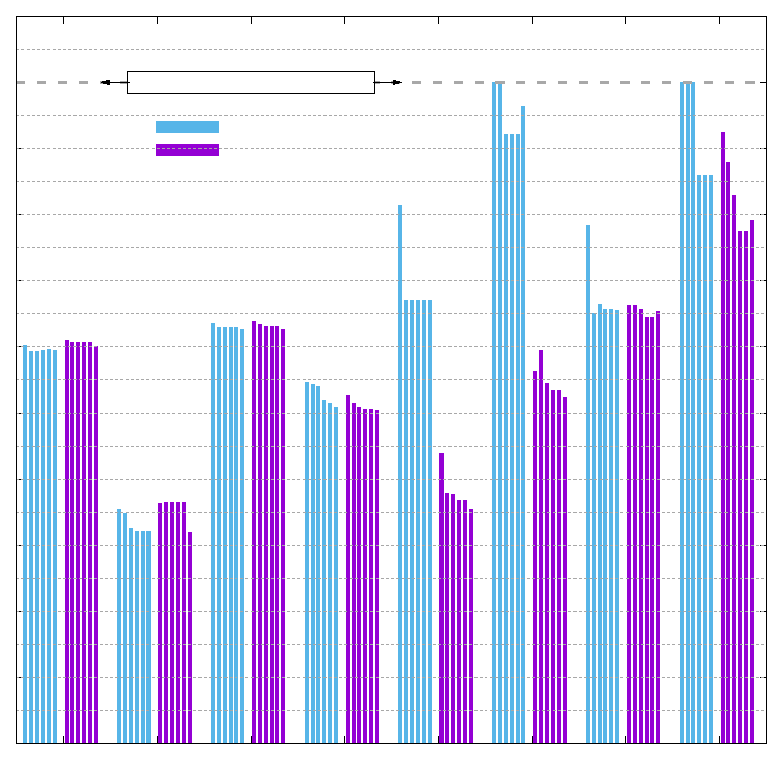
\includegraphics[width={360.00bp},height={360.00bp}]{abkm2020fig8}}%
    \gplfronttext
  \end{picture}%
\endgroup
